\chapter{Results}
\section{Segmentation}
The measures described in Section~\ref{sec:carotid} significantly improved carotid segmentation by effectively excluding brain lesions and undesired venous structures.
As illustrated in Figure~\ref{fig:seg_compare}, the cuboid mask plays a crucial role in this process.
Because no ground truth segmentation is available, visual inspection was used to evaluate the results, which showed that lesions and venous structures were rarely selected by the algorithm.
However, the algorithm was sometimes overly conservative.
In some instances, even when no non-carotid tissues were selected, parts of the carotid were inadvertently excluded.

\begin{figure}[h]
	\centering
	\begin{subfigure}{0.45\textwidth}
		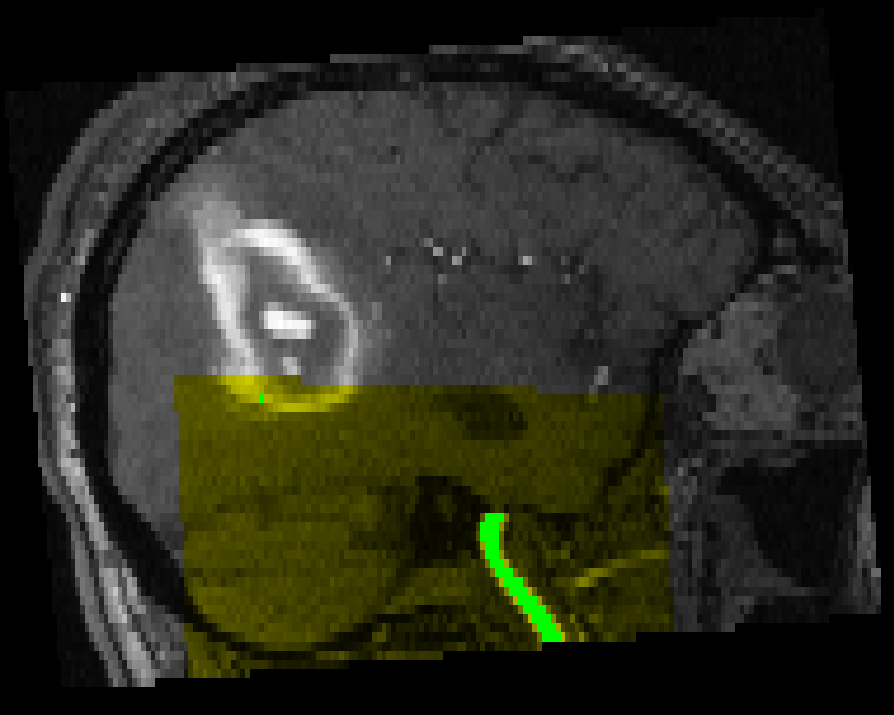
\includegraphics[width=\textwidth]{figures/molgu07704_bbox.png}
		\caption{}
		\label{subfig:seg_bbox}
	\end{subfigure}
	\begin{subfigure}{0.45\textwidth}
		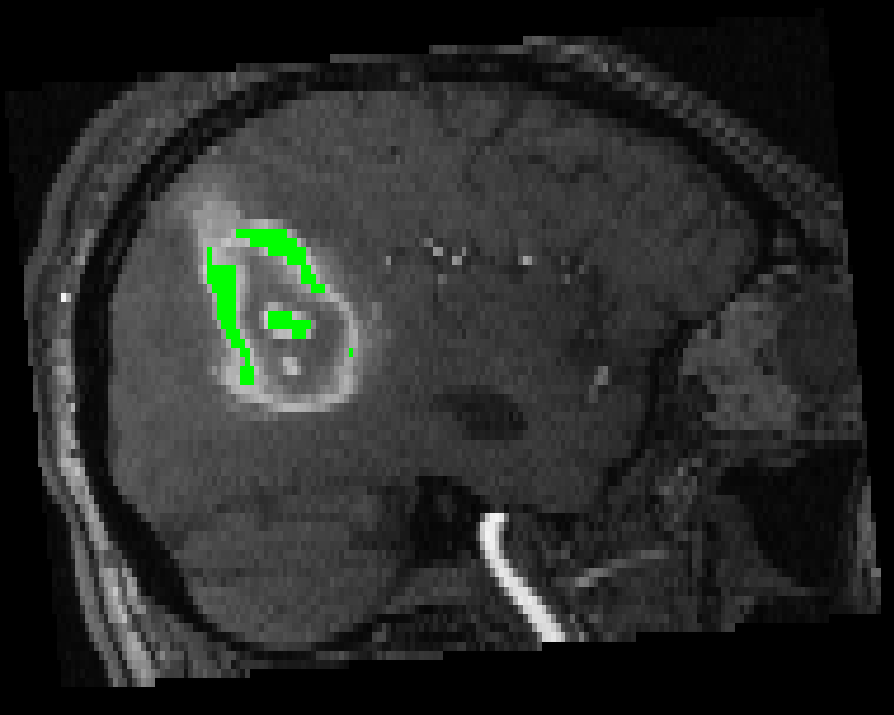
\includegraphics[width=\textwidth]{figures/molgu07704_nobbox.png}
		\caption{}
		\label{subfig:seg_nobbox}
	\end{subfigure}
	\caption{Comparison of carotid segmentation (green) with (a) and without (b) a cuboid mask (yellow). In the absence of the cuboid mask, the segmentation algorithm fails to capture the carotid and instead incorrectly identifies the brain lesion}
	\label{fig:seg_compare}
\end{figure}

\section{IDIF}
IDIF estimation was performed using both the Bayesian GTM (BGTM) and the conventional GTM PVC method.
The average mean absolute error (MAE) of the cumulative area under the curve (cAUC) across the dataset was 14,202 for BGTM and 33,764 for GTM.

ROI-based quantification was carried out using both IDIF methods, with BGTM yielding significantly better performance.
Specifically, the BGTM and GTM methods achieved an average \(\mrglu\) mean absolute percentage error (MAPE) of 14.1\% and 33\%, respectively, and an average \(\mrglu\) mean absolute error (MAE) of 1.42 and 3.5.
In addition, the MAE for the coefficient of determination (\(R^2\)) and the regression slope (\(S\)) were 0.004 and 0.14 for BGTM, compared to 0.030 and 0.304 for GTM, respectively.


\begin{table}[h]
	\centering
	\begin{tabular}{l|cc|cc}
		\toprule
		\multirow{2}{*}{\textbf{Metric}} & \multicolumn{2}{c|}{\textbf{BGTM}} & \multicolumn{2}{c}{\textbf{GTM}}                        \\
		\cmidrule(lr){2-3} \cmidrule(lr){4-5}
		                                 & \(\mu\)                            & \(\sigma\)                       & \(\mu\) & \(\sigma\) \\
		\midrule
		cAUC MAE                         & 14,202                             & 9,190                            & 33,764  & 21,212     \\
		\(\textrm{MR}_{glu}\) MAPE (\%)  & \textbf{14.1}                      & \textbf{10.1}                    & 33.0    & 31.5       \\
		\(\textrm{MR}_{glu}\) MAE        & 1.42                               & 1.07                             & 3.50    & 3.38       \\
		\(R^2\) Error                    & 0.004                              & 0.006                            & 0.030   & 0.132      \\
		Slope Error                      & 0.14                               & 0.109                            & 0.304   & 0.230      \\
		\bottomrule
	\end{tabular}
	\caption{Summary of performance metrics for BGTM and GTM methods.}
	\label{tab:metrics}
\end{table}

\begin{figure}[h]
	\centering
	\begin{subfigure}[b]{0.45\textwidth}
		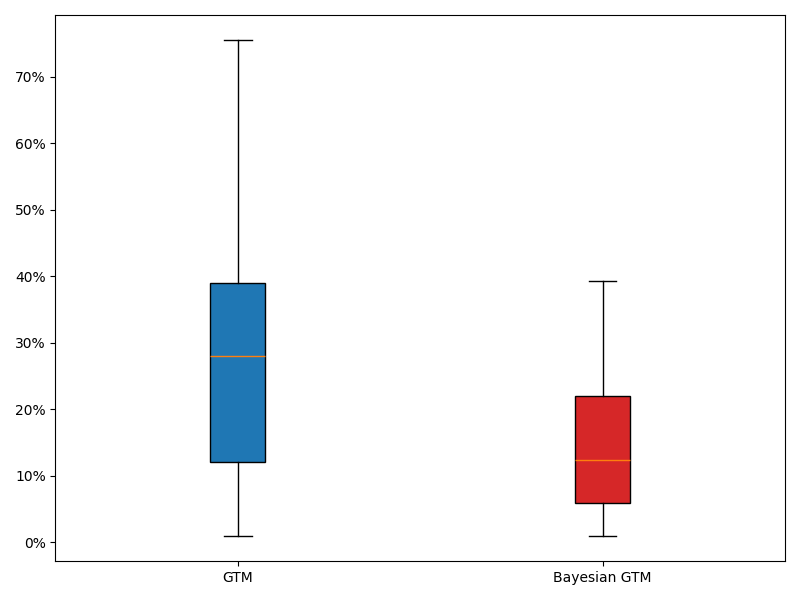
\includegraphics[width=\textwidth]{figures/quantification_mape_fitk3_boxplot.png}
		\caption{\(\mrglu\) MAPE Boxplot}
		\label{subfig:fitk3_mape}
	\end{subfigure}
	\begin{subfigure}[b]{0.45\textwidth}
		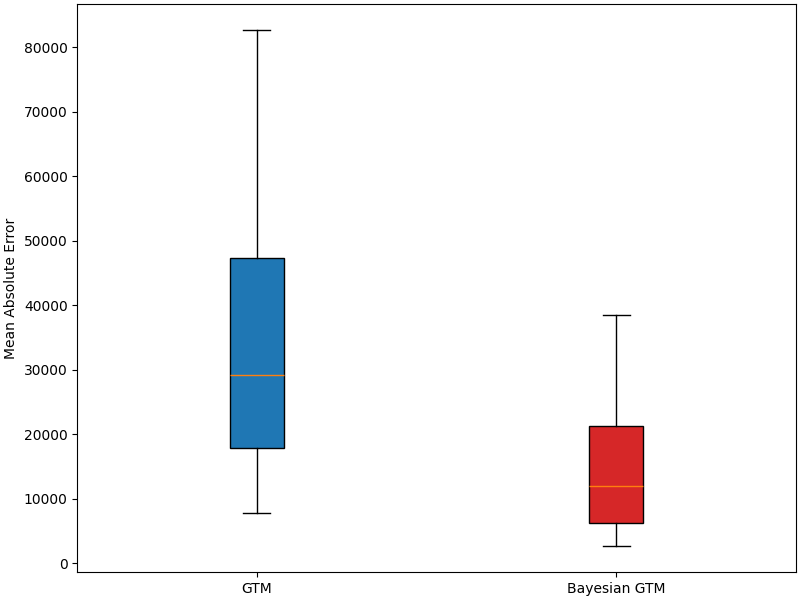
\includegraphics[width=\textwidth]{figures/curve_errors_boxplots.png}
		\caption{cAUC MAE Boxplot}
		\label{subfig:curve_errors_boxplot}
	\end{subfigure}
	\label{fig:boxplots}
	\caption{Boxplot of curve and quantification errors}
\end{figure}

As illustrated in Figure~\ref{fig:corr_mat}, there is a strong correlation between the MAE of the cAUC error and the quantification errors showing cAUC can be a good intermediate metric.
\pdfcomment{convincing enough reason?}

\begin{figure}[h]
	\centering
	\begin{subfigure}{0.45\textwidth}
		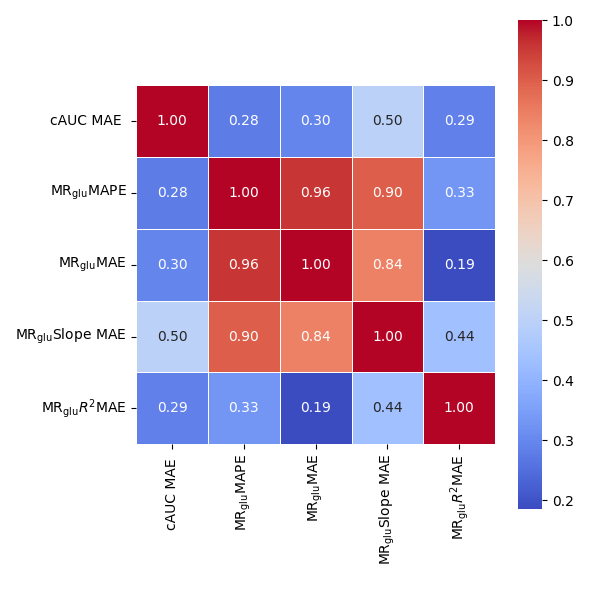
\includegraphics[width=\textwidth]{figures/corr_gtm.png}
		\caption{GTM}
		\label{subfig:corr_gtm}
	\end{subfigure}
	\begin{subfigure}{0.45\textwidth}
		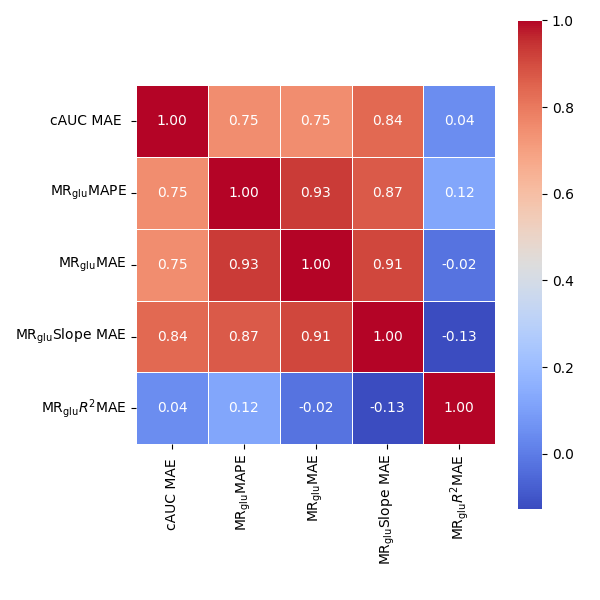
\includegraphics[width=\textwidth]{figures/corr_bgtm.png}
		\caption{Bayesian GTM}
		\label{subfig:corr_bgtm}
	\end{subfigure}
	\label{fig:corr_mat}
	\caption{Correlation matrix of different metrics for Bayesian GTM and GTM methods}
\end{figure}
\begin{figure}
	\centering
	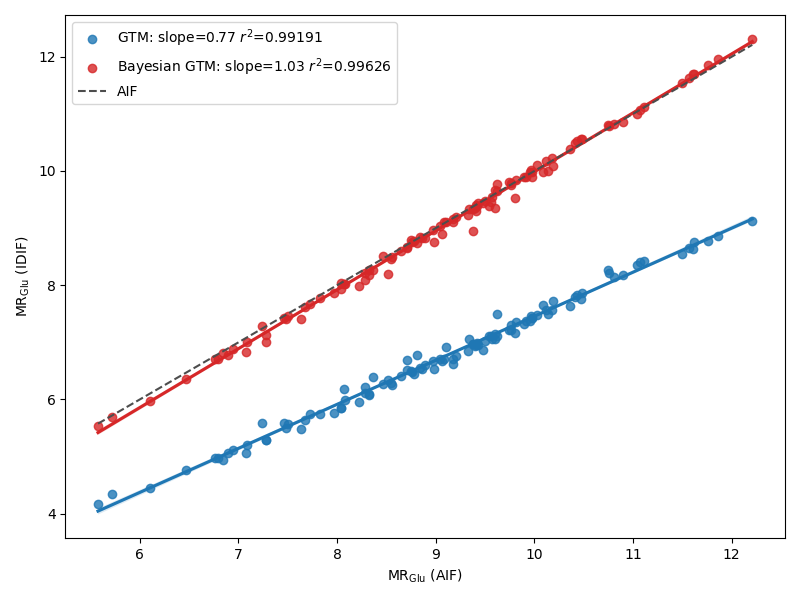
\includegraphics[width=0.55\textwidth]{figures/RD11934_1_cmrglu.png}
	\caption{\(\mrglu\) regression line for a specific subject}
\end{figure}
\begin{figure}
	\centering
	\begin{subfigure}{\textwidth}
		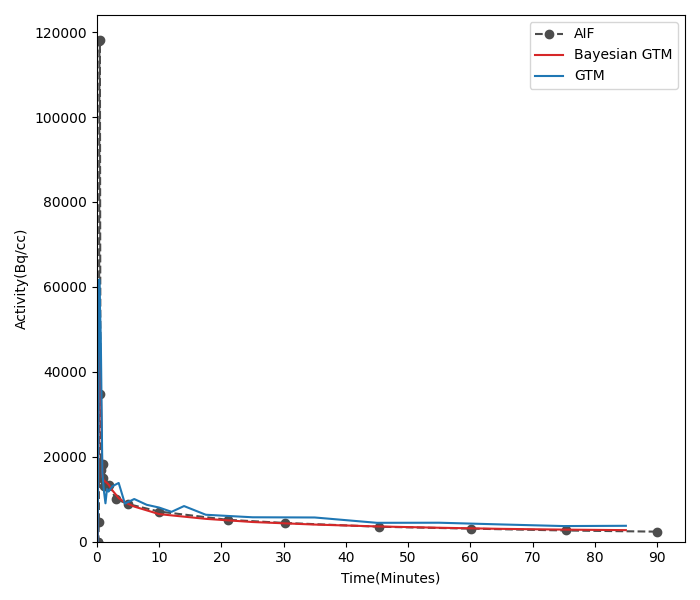
\includegraphics[width=\textwidth]{figures/RD11934_1_if_comparison.png}
		% \caption{Input function comparison}
		\label{subfig:if_compare}
	\end{subfigure}
	\begin{subfigure}{\textwidth}
		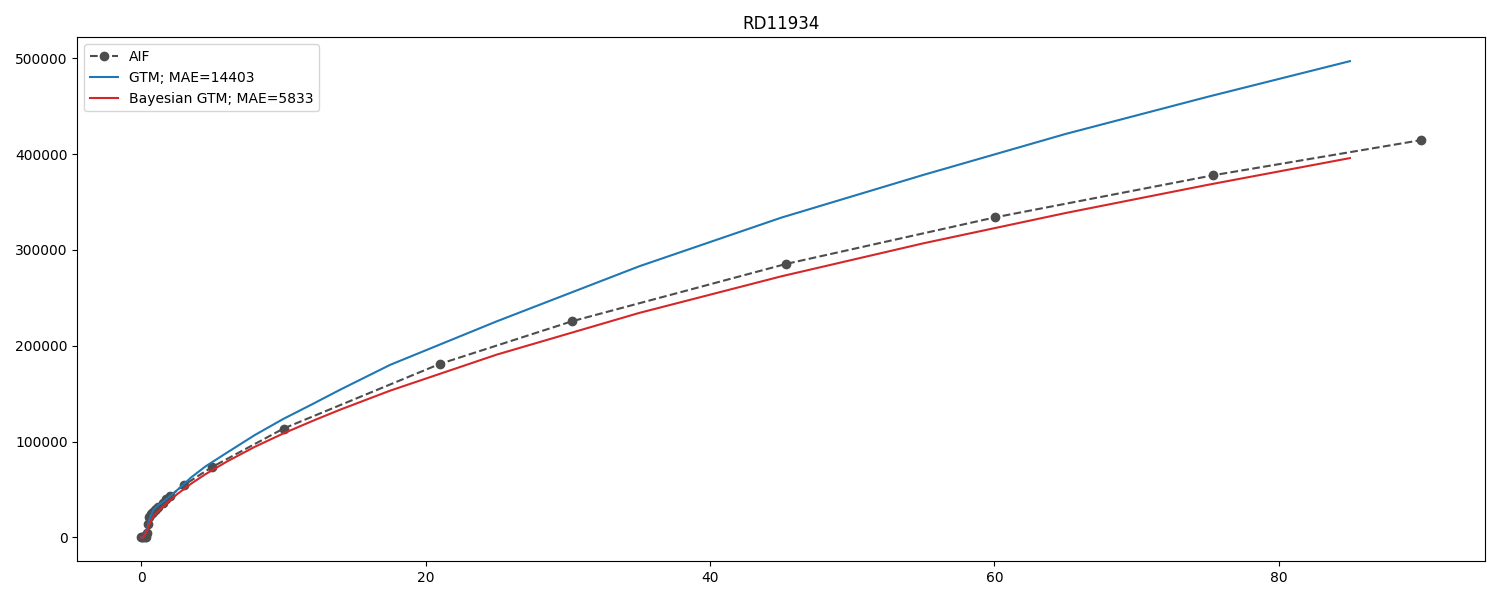
\includegraphics[width=\textwidth]{figures/RD11934_1_trap.png}
		% \caption{Cumulative AUC of IFs}
		\label{subfig:trap_compare}
	\end{subfigure}
	\label{fig:ifs}
	\caption{Comparison of the IFs (Top) and Cumulative AUC curves (Bottom) for a specific subject}
\end{figure}


